\documentclass[iop, usenatbib]{emulateapj}

%\documentclass{article}
\usepackage{amssymb}
\usepackage{epsfig}
\usepackage{color}
\usepackage{bm}
\usepackage{mathtools}
\usepackage{graphicx}
\usepackage{gensymb}
\usepackage{lipsum}
%\usepackage[showframe]{geometry}% http://ctan.org/pkg/geometry
%\usepackage{multicol}% http://ctan.org/pkg/multicols

\newcommand{\be}{\begin{equation}}
\newcommand{\ee}{\end{equation}}

%\slugcomment{ }
%\shorttitle{Polarization from neutron stars}
%\shortauthors{Me}

%\voffset=-1cm

\begin{document}
\title{Polarized adiation from rapidly rotating oblate neutron stars}

\author{M. M. Bigboy }

%\institute{ Me Me Big Boy}

\date{Received XXX / Accepted XXX}



\begin{abstract}
In this report the radiation escaping a plane-parallel electron consisting neutron star atmosphere is described.
The polarization plane rotation due to relativistic effects along the path from the star surface to the observer are described in terms of Tuomo's manuscript. 
Also the numeric methods for computing flux and polarization degree of outgoing from the star surface radiation are described. 
\lipsum[1]
\end{abstract}


\keywords{polarization --- numerical methods}

%\titlerunning{Meme BB}

\maketitle

\section{Polarization angle and polarization degree}
\subsection{Polarization angle }
At first we introduce the main polarization basis:
\be
\bm{e}_1^m = \frac{\bm{z}-\cos{i} \bm{k}}{\sin{i}},\qquad 
\bm{e}_2^m = \frac{\bm{k} \times \bm{z}}{\sin{i}},
\ee
which is fixed in the laboratory frame since the vector $\bm{e_1^m}$ is co-directed with the pulsar rotation axis.
The vector $\bm{z}$ or $\bm{\hat{\omega}}$ is the unit vector directed along the star spin axis.
Further we introduce the polarization basis formed by local normal $\bm{n}$ and the direction to the observer $\bm{k}$, in which the polarization vector will be lying in case of slowly rotating star (without relativistic rotation of the  polarization plane). 

\be
\bm{e}_1 = \frac{\bm{n}-\cos{\psi} \bm{k}}{\sin{\psi}},\qquad 
\bm{e}_2 = \frac{\bm{k} \times \bm{n}}{\sin{\psi}} .
\ee
This basis is rotating in relation to the previous one. The difference between polarization angleas in these two bases is called $ \chi _0 $ and is measured from the vector $\bm{e_1^m}$ to the $\bm{e_1}$  in the counterclockwise direction. Then we have:
$$
\cos{\chi}=\bm{e}_1^m \cdot \bm{e}_1 = \frac{\sin{i}\cos{\lambda}-\sin{\lambda}\cos{i}\cos{\varphi}}{\sin{\psi}} , 
$$\be
\sin{\chi}=\bm{e}_2^m \cdot \bm{e}_1 = - \frac{\sin{\lambda}\sin{\varphi}}{\sin{\psi}} ,
\ee
where the angle $\lambda=\theta-\gamma$ is the angle between radius vector $\bm{r}$ and the local normal vector $\bm{n}$. By these values the angle $\chi$ can be unambiguously identified. To take into account the polarization plane rotation due to relativistic  motion, we now introduce the another basis. This basis is related to the local (when it is close to the neutron star surface) photon direction  $\bm{k_0}$:
\be
\bm{e}_1^0 = \frac{\bm{n}-\cos{\sigma} \bm{k_0}}{\sin{\sigma}},\qquad 
\bm{e}_2^0 = \frac{\bm{k_0} \times \bm{n}}{\sin{\sigma}} .
\ee
One can notice that $\bm{e}_2^0 =\bm{e}_2$. This equation is due to the fact that photon trajectories are planar. 
If in the spot rest frame the polarization vector lies in the meridional plane, which is described by $\bm{e}_1^0$ component, then it will be transformed to (Nagirner, Poutanen '93)
\be
\bm{e}_1' = \frac{\bm{n}-\delta\gamma\cos{\sigma} (\bm{\beta-k_0})}{\sqrt{1-\delta^2 \cos^2{\sigma} } }
\ee
in the non-rotating frame. The relativistic rotation of the polarization vector is given by the angle $\chi'$. If we denote $\eta=\delta\cos{\sigma}$ and $\bm{\beta}=\bm{\hat\beta} \beta$, where $\bm{\hat\beta}$ is a unit vector of velocity, then we can put
\be
\sin{\chi'}=\bm{e}_1'\cdot \bm{e}_2^0 =
 \frac{\eta\gamma\beta }{\sin{\sigma}\sqrt{1-\eta^2} } \bm{\hat\beta} \cdot(\bm{k_0} \times \bm{n}),
\ee
from where $\bm{\hat\beta} \cdot(\bm{k_0} \times \bm{n}) $ transforms into 
\be
 \bm{k_0} \cdot (\bm{n}\times\bm{\hat\beta} )=
 \bm{k_0} \cdot \left(\bm{n} \times \frac{\bm{n} \times \bm{r}}{\sin{\gamma}}\right)=\ee$$
 \bm{k_0} \cdot \frac{\cos{\gamma}\bm{n} - \bm{r}}{\sin{\gamma}} =
 \frac{\cos{\sigma}\cos{\gamma}-\cos{\alpha}}{\sin{\gamma}},
$$

and then we eventually have \be
\sin{\chi'}=\bm{e}_1'\cdot \bm{e}_2^0 =
 \frac{\eta\gamma\beta (\cos{\sigma}\cos{\gamma}-\cos{\alpha})}{\sin{\gamma}\sin{\sigma}\sqrt{1-\eta^2} }.
\ee
But in the case of a spherical star $\gamma$ is always equal to $0$. 
Then one can derive another formula for the triple product:

\be
 \bm{k_0} \cdot (\bm{n}\times\bm{\hat\beta} )= -\bm{m} \cdot \bm{k_0}  = 
\ee$$
 \frac{ (\sin{i}\cos\lambda\cos\phi-\cos{i}\sin\lambda)\sin\alpha + \sin{(\psi-\alpha)}}{\sin{\psi}}
$$

For the cosine of the angle  $\chi'$ one can simply use  Pythagorean trigonometric identity $\cos{\chi'}=\sqrt{1-\sin^2{\chi'}}$ for one of the previous expressions for $\sin{\chi'}$ or make the next derivation: 
$$
\cos{\chi'}=\bm{e}_1'\cdot \bm{e}_1^0 = 
 \frac{\bm{n}-\eta\gamma (\bm{\beta-k_0})}{\sqrt{1-\eta^2 } } \cdot 
\frac{\bm{n}-\cos{\sigma} \bm{k_0}}{\sin{\sigma}}=$$$$
 \frac{1 + \beta\gamma\eta\cos\sigma\cos\xi-\cos^2 \sigma}{\sin\sigma\sqrt{1-\eta^2}} =
 \frac{\sin^2 \sigma + \beta\gamma\eta\cos\sigma\cos\xi}{\sin\sigma\sqrt{1-\eta^2}}=$$\be
 \frac{\sin^2 \sigma + \beta\gamma\eta\cos\sigma\sin\alpha\sin\varphi\sin{i}/\sin\psi}{\sin\sigma\sqrt{1-\eta^2}}
 \ee
And then reduce to an expression for $\chi'$\be
\tan\chi' 
= \eta\gamma\beta \ee$$\times 
\frac{
 (\sin{i}\cos\lambda\cos\phi-\cos{i}\sin\lambda)\sin\alpha + \sin{(\psi-\alpha)}
}{
\sin\psi\sin^2 \sigma + \beta\gamma\eta\cos\sigma\sin\alpha\sin\varphi\sin{i}
}
$$
Finally, the total polarization angle of radiation from one point on the surface is\be
\chi=\chi_0+\chi'\ee

\subsection{Polarization degree}
Since we do not consider circular polarization, the Stokes vector contains three components $(F_I,F_Q,F_U)$.
In the last polarization basis, the polarization angle will always equal to 0, because of axial symmetry of the neutron star, and then $F_U$ will be also always zero. Polarization degree $P$ in this case is determined by  $F_Q=P F_I$, and will not change if the polarization basis rotates. When we rotate the Stokes vector to the main basis, we get the result vector $$(F_I, F_Q \cos{2\chi},F_Q \sin{2\chi}),$$   

The total Stokes vector is obtained from summing the vectors for primary and secondary spots (denoted by indexes $tot$, $p$ and $s$ respectively) if there are two spots on the neutron star, and if the spots are big enough that we not neglect their sizes anymore, we should sum Stokes vector for several points in the area of the spot$$
F_I^{tot}=F_I^p+F_I^s = \sum_i F_I^{p,i}+F_I^{s,i}$$\be
F_Q^{tot}=F_Q^p+F_Q^s = \sum_i F_Q^{p,i}+F_Q^{s,i}\ee$$
F_U^{tot}=F_U^p+F_U^s= \sum_i F_U^{p,i}+F_U^{s,i} $$\be
P^{tot}=\frac{\sqrt{(F_Q^{tot})^2+(F_U^{tot})^2}}{F_I^{tot}}\ee
And for multiple points on the surface we can obtain the total polarization angle from the total Stokes vector\be
\tan{2\chi^{tot}}=\frac{F_U^{tot}}{F_Q^{tot}}\ee

\subsubsection{X-ray bursts}
Further some results (figures \ref{figure:angswap}, \ref{figure:sizedif} and \ref{figure:freqdif})are obtained using approximate formula of dependence of the polarization degree on $\mu=\cos{\sigma}$  during the X-ray burst
\be
P=-\frac{1-\mu}{1+3.582\mu}11.71\%
\ee
The direction of the electric vector oscillations is perpendicular to the meridional plane.
The formula was obtained approximating the solution for the plane parallel semi-infinite atmosphere with opacity dominated by Thomson scattering.

\begin{figure} 
 \centering
 \includegraphics[width=.5\textwidth]{test2.eps}
 \caption{The dependency on angular configuration. On this figure the two situations are shown: basic, $\theta=20\degree,\, i=40\degree$ and swapped, $\theta=40\degree,\, i=20\degree$. For such an angles permutation the energy fluxes would be the same, but it is important that these two situations be told apart, and we can distinguish them by the polarization angle curves. On the figure by the solid and dashed lines the polarization degrees are shown in percents for the two cases respectfully and by the dotted and dash-dot lines the polarization angles are shown respectfully as well.The basic set of parameters is $\rho=1\degree,\, \nu = 600$ Hz, $ R=2.5 r_g ,\, M=1.4 M_{\odot}$.  }
 \label{figure:angswap}
\end{figure}

\begin{figure}
 \centering 
 \includegraphics[width=0.5\textwidth]{test1.eps}
 \caption{The dependency on spot size is shown by comparison spots of the angular sizes $(\rho=1\degree)$ and $(\rho=20\degree)$.  By the solid and dashed lines the polarization degrees are shown in percents  for  the small (basic) and the big spots respectfully. By the dotted and dash-dot lines the polarization angles are shown respectfully as well.}
 \label{figure:sizedif}
\end{figure}
 

\begin{figure}
 \centering
 \includegraphics[width=0.5\textwidth]{test3.eps}
 \caption{The dependency on spin is shown by comparison the $\nu=600$ Hz and $\nu=1$Hz frequencies. By the solid and dashed lines the polarization degrees are shown in percents for the big spin (basic) and the slow rotating stars respectfully.    By the dotted and dash-dot lines the polarization angles are shown respectfully as well.}
 \label{figure:freqdif}
\end{figure}

\subsubsection{Thomson scattering}
The intensity of unscattered photons is
\be
I_{l,r}^0=I_{in}e^{-\tau/\mu}
\ee
The boundary conditions for $n$ times scattered photons are
\be
I_{l,r}^n(\tau=0,\mu)=I_{l,r}^n(\tau=\tau_T,-\mu)=0\qquad 0\leq\mu\leq1
\ee
The intensity of $n$ times scattered photons are computedfrom
$$
I_l^n(\tau,\mu)=\int_{\tau_b(\mu)}^\tau \frac{d\tau'}\mu e^{\frac{\tau'-\tau}\mu}$$\be
\times( A^n(\tau')(1-\mu^2) + (B^n(\tau')+C^n(\tau')\mu^2 ),
\ee$$
I_l^n(\tau,\mu)=\int_{\tau_b(\mu)}^\tau \frac{d\tau'}\mu e^{\frac{\tau'-\tau}\mu}
(B^n(\tau')+C^n(\tau'))
$$
where $$
A^n(\tau)=\frac34\int_0^1 d\mu' (I^{n-1}_l (\tau,\mu')+I^{n-1}_l (\tau,-\mu')) (1-\mu'^2)
$$\be
B^n(\tau)=\frac38\int_0^1 d\mu' (I^{n-1}_l (\tau,\mu')+I^{n-1}_r (\tau,-\mu'))\mu'^2
\ee$$
C^n(\tau)=\frac38\int_0^1 d\mu' (I^{n-1}_r (\tau,\mu')+I^{n-1}_r (\tau,-\mu')) 
$$

Then one can compute the intensity of escaping photons\be
I(\mu)=I_l(\tau_T,\mu)+I_r(\tau_T,\mu)
\ee
and the polarization degree of the outgoing radiation (see Figure \ref{figure:ThomsonIp})
\be
p(x,\mu)
=\frac{I_l(\tau_T,\mu)+I_r(\tau_T,\mu)}{I_l(\tau_T,\mu)-I_r(\tau_T,\mu)}
=100\%\frac{I(\mu)}{Q(\mu)}.\ee


\begin{figure}
 \centering
 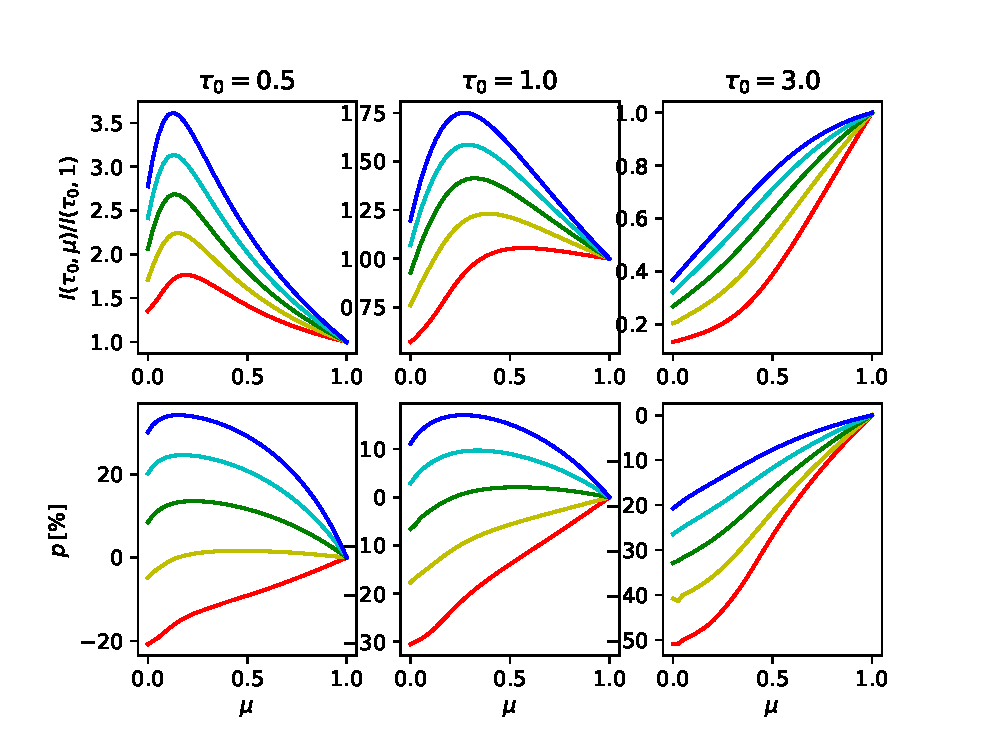
\includegraphics[width=0.5\textwidth]{Ip.eps}
 \caption{Intensity normalized to unity at $\mu=1$ and polarization degree of the outgoing from plane parallel slab (for several different Thomson optical depths $\tau_T=0.5,\,1.0,\,3.0$) photons
  that have undergone 1, 2, 3, 4 and 5 scatterings (red, yellow, green, cyan and blue lines respectfully)} 
 \label{figure:ThomsonIp}
\end{figure}

But these functions have no dependence on frequencies, while in neutron stars the electron momenta are big enough to change energies of the photons. It means that Compton scattering must be taken into account.

\subsubsection{Compton scattering}
The computing of Compton scattering in a plane-parallel infinite slab is discussed  not here yet



 


\end{document}

